\documentclass[10pt]{article}
\usepackage[right=2cm,left=2cm,top=2cm,bottom=3cm]{geometry}
\usepackage[utf8]{inputenc}
\usepackage[spanish]{babel}
\usepackage{amsmath}
\usepackage{color}
\usepackage{listings}
\usepackage{graphicx}
%\usepackage{multicol}

%COLORES CODIGO
\definecolor{gray97}{gray}{.97}
\definecolor{gray75}{gray}{.75}
\definecolor{gray45}{gray}{.45}
\definecolor{claregreen}{RGB}{4,180,95}
\definecolor{darkblue}{rgb}{0.0,0.0,0.6}


\lstset{ frame=Ltb,
     framerule=0pt,
     aboveskip=0.5cm,
     framextopmargin=3pt,
     framexbottommargin=3pt,
     framexleftmargin=0.4cm,
     framesep=0pt,
     rulesep=.4pt,
     backgroundcolor=\color{gray97},
     rulesepcolor=\color{black},
     %
     stringstyle=\ttfamily,
     showstringspaces = false,
     basicstyle=\small\ttfamily,
     commentstyle=\color{gray45},
     keywordstyle=\bfseries,
     %
     numbers=left,
     numbersep=15pt,
     numberstyle=\tiny,
     numberfirstline = false,
     breaklines=true,
   }

% minimizar fragmentado de listados
\lstnewenvironment{listing}[1][]
   {\lstset{#1}\pagebreak[0]}{\pagebreak[0]}

%LENGUAJE OZ
\lstdefinelanguage{OZ}
{
  morestring=[b]',
  morecomment=[s]{\%}{\%},
  stringstyle=\color{claregreen},
  keywordstyle=\color{blue}\bfseries,
  morekeywords={proc, end, \$},% list your attributes here
  emph={REQUIRED},
  emphstyle=\color{red}
}

%MODO CONSOLA
\lstdefinestyle{consola}
   {basicstyle=\scriptsize\bf\ttfamily,
    backgroundcolor=\color{gray75},
   }


\title{ \textbf{Modelo Matemático para la Acomodación de un Basurero en una Ciudad.}}

\author{Maria Andrea Cruz Blandón 0831816 \and Edgar Andrés Moncada  Taborda 0832294 \and Hebert Vargas Tello 1124798 \and Luis Felipe Vargas Rojas 0836342  }

\date{Enero 2013}

\begin{document}
\maketitle

\tableofcontents

\newpage

\section{Introducci\'on}
En el siguiente documento se explicará el modelo construido a través del paradigma de la programación linea (lp), para resolver el problema de la acomodación de un basurero en una ciudad, el problema se basa en que la construcci\'on del basurero se debe realizar en el lugar  m\'as alejado posible de la ciudad más cercana, esto debido a los malos olores que genera y a las molestias de cada ciudad por dicha construcción.\\

Los principales problemas a los que nos enfentramos al tratar de modelar este problema con lp fueron  definir los dominios las variables, establecer una forma para definir distancias entre ciudades y el basurero a trav\'es de un valor absoluto, definir a través de restricciones la ciudad m\'as cercana entre otros detalles que se explicarán en el documento.\\

Para la implementación del modelo usamos el programa lpsolve y una librería de java que genera el archivo de entrada para el lpsolve teniendo en cuenta los valores de entrada.

\section{Modelo Programaci\'on Lineal} 

\subsection{Datos de Entrada}
\begin{tabular}{l l }
$T$ & Tamaño de la grilla (T x T)\\
$N$ & Numero de ciudades.\\ 
$X_i$ & Coordenada x de la ciudad i. \\
$Y_i$ & Coordenada y de la ciudad i. \\

\end{tabular}


\subsection{Variables del Problema}
\begin{tabular}{p{1cm} p{0.9\textwidth}}
$Xb$ & Coordenada x del basurero \\
$Yb$ & Coordenada y del basurero \\
$Xc$ & Coordenada x de la ciudad m\'as cercana al basurero \\
$Yc$ & Coordenada y de la ciudad m\'as cercana al basurero \\
$Zx_i$ & Diferencia entre la coordenada x del basurero ($Xb$) y la coordenada x de la ciudad i\\
$Zy_i$ & Diferencia entre la coordenada y del basurero ($Yb$) y la coordenada y de la ciudad i\\
$Zx_ia$ & Usada para el valor absoluto de la diferencia entre entre la ciudad i y el basurero representa la parte positiva de la variable $Zx_i$\\
$Zx_ib$ & Usada para el valor absoluto de la diferencia entre la ciudad i y el basurero, representa la parte negativa de la variable $Zx_i$\\
$Zy_ia$ & Usada para el valor absoluto de la diferencia entre la ciudad i y el basurero representa la parte positiva de la variable $Zy_i$\\
$Zy_ib$ & Usada para el valor absoluto de la diferencia entre la ciudad i y el basurero representa la parte negativa de la variable $Zy_i$\\
$dx$ & Diferencia entre $Xc$ - $Xb$ \emph{Usado para la funci\'on objetivo}\\
$dy$ &  Diferencia entre $Yc$ - $Yb$ \emph{Usado para la funci\'on objetivo}\\
$Zx$ & Valor absoluto de $dx$\\
$Zy$ & Valor absoluto de $dy$ \\
\end{tabular}


\subsection{Variables Binarias del Problema}
\textbf{Usadas para el Valor Absoluto de la Diferencia de cada Ciudad con el Basurero: }\\

\begin{tabular}{l l }
 $Bx_{ia}$ & Usada en las restricciones del valor absoluto para la ciudad i coordenada x \\
$Bx_{ib}$ & Usada en las restricciones del valor absoluto para la ciudad i  coordenada x \\
$By_{ia}$ & Usada en las restricciones del valor absoluto para la ciudad i coordenada y \\
$By_{ib}$ & Usada en las restricciones del valor absoluto para la ciudad i coordenada y \\

\end{tabular}\bigskip 

\textbf{Usadas para  que  $Xc \in X_i$ y $Yc \in Y_i$.}\\

\begin{tabular}{l l }
$Bc_i$ & Toma el valor de 1 si la ciudad i es la m\'as cercana \\
\end{tabular}\bigskip


\textbf{Usadas para  el valor absoluto de la funci\'on objetivo.}\\


\begin{tabular}{l l }
$Bx0$ &   Usada para el valor absoluto en la función objetivo coordenada x \\
$By0$ &   Usada para el valor absoluto en la función objetivo coordenada y \\
\end{tabular}\bigskip



\subsection{Restricciones Obvias}
\textbf{Dominios de las Variables}\\

\begin{center}
 $0$ $\leq $ $Xb$,$Yb$,$Xc$,$Yc$, $Zx$, $Zy$  $\leq $ $T$
 
 $Zx_i$ , $Zy_i$ Son variables irrestrictas.
\end{center}

\subsection{Restricciones del Problema}
\textbf{Garantizar que:  $Xc \in X_i$ y $Yc \in Y_i$. }\\

\begin{center}
$Xc$ = $\sum_i X_i * Bc_i$

$Yc$ = $\sum_i Y_i * Bc_i$

$\sum_i Bc_i = 1$

$i \in [1,N]$

 \emph{En la implementación se debe normalizar las restricciones por eso la sumatoria pasa al otro lado a restar y queda igual a cero la restricci\'on, esto se hace con todas las restricciones.}

\end{center}


\textbf{Diferencias de distancias entre el basurero y la ciudad i, $Zx_i$,$Zy_i$ }\\

\begin{center}

 $Zx_i$ = $X_i- Xb $ 
 
  $Zy_i$ = $Y_i-Yb$ 
  
  $i \in [1,N]$
\end{center}

\textbf{Valor absoluto para  $Zx_i$,$Zy_i$ }\\

\begin{center}

 $Zx_i$ = $Zx_ia  - Zx_ib$ 
 
  $Zy_i$ = $Zy_ia  - Zy_ib$ \medskip 
  
  $M*Bx_{ia} - Zx_ia >= 0$
  
  $M*By_{ib} - Zy_ib >= 0$\medskip 
  
  $ Bx_{ia} + Bx_{ib} = 1 $
  
  $ By_{ia} + By_{ib} = 1 $\medskip 
  
   $i \in [1,N]$
   
   $M=T+1$\bigskip
  
   $ |Zx_i|=Zx_ia  + Zx_ib $ 
   
   $ |Zy_i|=Zy_ia  +  Zy_ib $ 
\end{center}


\textbf{Para que  $Zx$,$Zy$  tomen los valores de la ciudad más cercana al basurero se debe cumplir que: }\\

\begin{center}

 
  $ |Zx_i| + |Zy_i| \geq Zx + Zy $
  
   
   $i \in [1,N]$
  
  

\end{center}


\textbf{Diferencia entre ciudad  m\'as cercana y basurero: }\\

\begin{center}

 
  $ dx = Xc - Xb $
  
   
   $dy = Yc - Yb$
  
  

\end{center}


\subsection{Funci\'on Objetivo.}

Para la funci\'on objetivo nos encontramos de nuevo con el problema del valor absoluto ya que calculamos diferencias y podemos obtener resultados con valores negativos.\\

La función objetivo definida es: 

\begin{center}
      MAX( $Zx + Zy$)
\end{center}

Donde $Zx$ y $Zy$ son la representaci\'on en valor absoluto de $dx$ y $dy$, respectivamente por lo cual ésta funci\'on objetivo está sujeta a : 

\begin{center}
$dx + MB - Zx \geq 0 $

$dx + MB + Zx \leq M $

$dx \leq Zx $

$-dx \leq Zx$

\end{center}


\begin{center}
$dy + MB - Zy \geq 0 $

$dy + MB + Zy \leq M $

$dy \leq Zy $

$-dy \leq Zy$

\end{center}

\newpage

\section{Branch and Bound}

Para la variables binarias que dan soporte a las restricciones relacionadas con los valores absolutos de las distancias y la función objetivo y que la ciudad más cercana corresponda
a una ciudad del problema. Para ver mayor información revisar la sección \textbf{Variables Binarias del Problema}.\\

Para el algoritmo \emph{Branch and Bound} (\textbf{B\&B}) usamos la implementación en la librería \emph{LpSolve}. Dicha librería trae varias heurísticas con las cuales usar
el B\&B, además de las heurísticas para elegir la rama a tomar, también esta disponible la opción de si iniciar la rama con la función techo o con la función piso.\\

De las heurísticas que están disponibles en \emph{LpSolve} elegimos 13 para comparar el rendimiento. Además por cada heurística ésta se probó con la función techo y la función piso, para 
evaluar la mejor combinación. A continuación se explica el proceder de las 13 heurísticas\footnote{fuente: http://lpsolve.sourceforge.net/5.5/set\_bb\_rule.htm}:

\begin{enumerate}
 \item \textbf{NODE\_FIRSTSELECT}: Elige la primera columna no entera.%1
 \item \textbf{NODE\_GAPSELECT}: Selecciona la variable de acuerdo a la distancia de los límites actuales.%2
 \item \textbf{NODE\_RANGESELECT}: Selecciona la variable de acuerdo al mayor límite actual.%3
 \item \textbf{NODE\_FRACTIONSELECT}: Selecciona la variable que tenga el valor fraccionario más grande.%4
 \item \textbf{NODE\_PSEUDOCOSTSELECT}: Selecciona la variable con la estrategia pseudo-costo (búsqueda costo uniforme)%5
 \item \textbf{NODE\_PSEUDONONINTSELECT}: Es una extensión de la estrategia pseudo-costo basada en minimizar el número de enteros fallidos.%6
 \item \textbf{NODE\_PSEUDORATIOSELECT}: También es una extensión de la estrategia pseudo-costo basada en maximizar la razón pseudo-cost divido por el número de fallidas. Similar a costo/beneficio.%7
 \item \textbf{NODE\_WEIGHTREVERSEMODE}: Selecciona la variable por el peor criterio en vez del mejor criterio.%8
 \item \textbf{NODE\_GREEDYMODE}: Búsqueda informada, con un costo heurístico.%9
 \item \textbf{NODE\_DEPTHFIRSTMODE}: Búsqueda en profundidad, selecciona el nodo por el que ya venia explorando.%10
 \item \textbf{NODE\_RANDOMIZEMODE}: Añade un factor random al costo de un nodo candidato.%11
 \item \textbf{NODE\_BREADTHFIRSTMODE}: Selecciona el nodo que no se halla seleccionado o que se halla seleccionado menos veces (anteriormente).%12
 \item \textbf{NODE\_AUTOORDER}: Crea una variable de ordenamiento ``óptima'' para el B\&B. (Indexación)%13
\end{enumerate}


Para realizar la pruebas correspondientes se generaron $20$ ejemplos aleatorios. 5 ejemplos con una grilla de tamaño $5$ y número de ciudades aleatorio, 5 ejemplos con una grilla
de tamaño $10$ y número de ciudades aleatorio, 5 ejemplo con una grilla de tamaño $15$ y número de ciudades aleatorio y 5 ejemplos con una grilla de tamaño $20$ y número de ciudades aleatorio.
A cada ejemplo se le aplica el algoritmo con cada heurística una vez con la función techo y otra con la función piso.\\

Comparamos el desempeño de las heurísticas usando la función techo con los 5 ejemplos de un tamaño de grilla y así con todos los tamaños de la grilla. Se comparaban las heurísticas en 3 tres grupos,
por cada grupo se seleccionaba la heurística con el mejor desempeño, y al final se eligió la mejor de las tres mejores. Este fue el procedimiento aplicado para las comparaciones por ejemplos. Finalmente
se realizó una comparación entre todos los ejemplos (se eligió el un ejemplo por cada tamaño de grilla, el que tuviera mas ciudades) para elegir las 3 mejores heurísticas, dichas heurísticas
usaban la función piso. \\


%%INICIA GRILLA 5

\newpage
\subsection{Ejemplos tamaño de grilla 5}

Gráficas correspondientes al desempeño de las heurísticas, 3 grupos:\\
\textbf{Usando techo:}


\begin{figure}[ht]
\begin{minipage}[b]{0.45\linewidth}
 \centering
 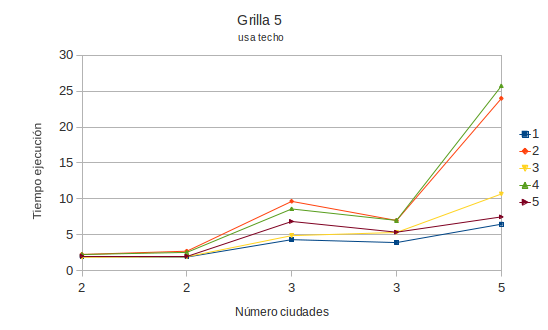
\includegraphics[width=\textwidth]{grilla5ceil0.png}
 % grilla5ceil0.png: 548x330 pixel, 72dpi, 19.33x11.64 cm, bb=0 0 548 330
 \caption{Comparación heurísticas  1 $\cdots$ 5}
 \label{fig:grid5ceil0}
\end{minipage}
\hspace{0.5cm}
\begin{minipage}[b]{0.45\linewidth}
 
\centering
 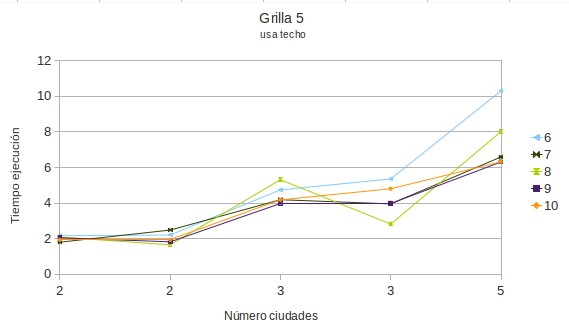
\includegraphics[width=\textwidth]{grilla5ceil1.png}
 % grilla5ceil0.png: 548x330 pixel, 72dpi, 19.33x11.64 cm, bb=0 0 548 330
 \caption{Comparación heurísticas  6 $\cdots$ 10}
 \label{fig:grid5ceil1}
\end{minipage}

\begin{minipage}[b]{1\linewidth}
  \centering
 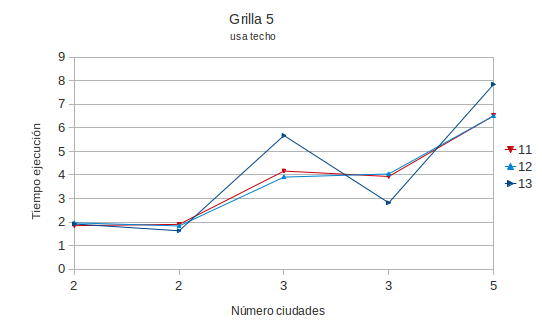
\includegraphics[scale=0.4]{grilla5ceil2.png}
 % grilla5ceil0.png: 548x330 pixel, 72dpi, 19.33x11.64 cm, bb=0 0 548 330
 \caption{Comparación heurísticas  11 $\cdots$ 13}
 \label{fig:grid5ceil2}
\end{minipage}

\end{figure}


De la figura \ref{fig:grid5ceil0} la heurística que presentó mejor desempeño fue la número $1$ (NODE\_FIRSTSELECT), de la figura \ref{fig:grid5ceil1} fue la número $9$ (NODE\_GREEDYMODE) y de la 
figura \ref{fig:grid5ceil2} fue la número $12$ (NODE\_BREADTHFIRSTMODE). Al comparar éstas tres, la mejor correspondió a la heurística número $9$ (NODE\_GREEDYMODE).

\begin{figure}[ht]
\begin{minipage}[b]{1\linewidth}
 \centering
 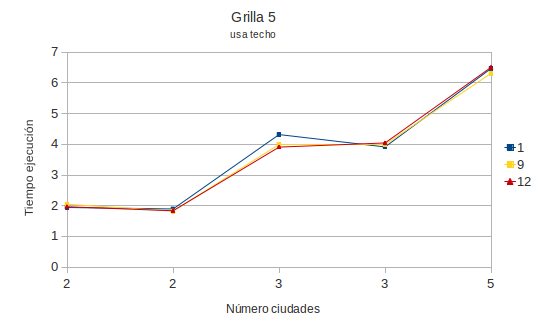
\includegraphics[scale=0.4]{grilla5ceil3.png}
 % grilla5ceil3.png: 539x326 pixel, 72dpi, 19.01x11.50 cm, bb=0 0 539 326
 \caption{Comparación mejor heurística}
 \label{fig:grid5ceil3}
\end{minipage}
\end{figure}


\newpage
\textbf{Usando piso:}

\begin{figure}[ht]

\begin{minipage}[b]{0.45\linewidth}
 \centering
 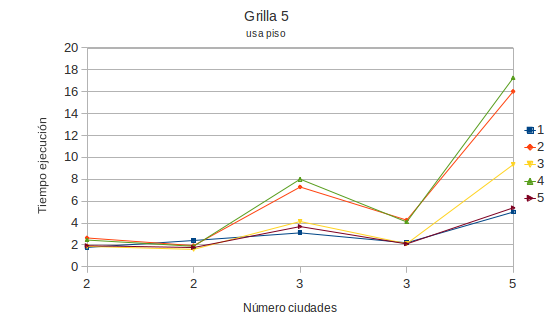
\includegraphics[width=\textwidth]{grilla5floor0.png}
 % grilla5ceil0.png: 548x330 pixel, 72dpi, 19.33x11.64 cm, bb=0 0 548 330
 \caption{Comparación heurísticas  1 $\cdots$ 5}
 \label{fig:grid5floor0}
\end{minipage}
\hspace{0.5cm}
\begin{minipage}[b]{0.45\linewidth}
 \centering
 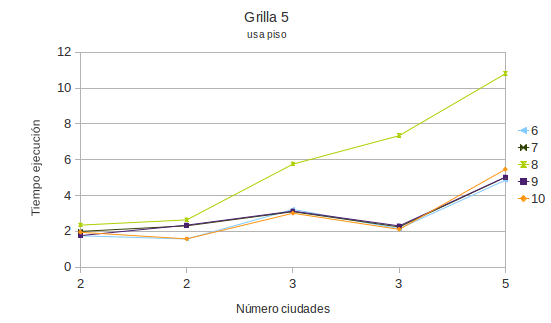
\includegraphics[width=\textwidth]{grilla5floor1.png}
 % grilla5ceil0.png: 548x330 pixel, 72dpi, 19.33x11.64 cm, bb=0 0 548 330
 \caption{Comparación heurísticas  6 $\cdots$ 10}
 \label{fig:grid5floor1}
\end{minipage}

\begin{minipage}[b]{1\linewidth}
  \centering
 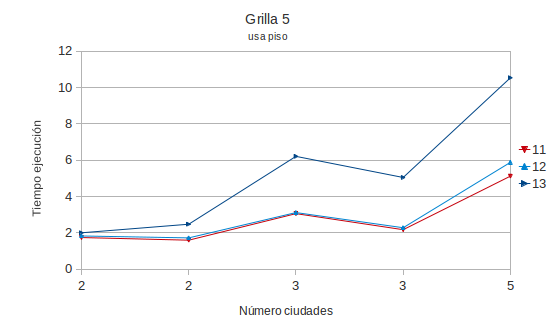
\includegraphics[scale=0.4]{grilla5floor2.png}
 % grilla5ceil0.png: 548x330 pixel, 72dpi, 19.33x11.64 cm, bb=0 0 548 330
 \caption{Comparación heurísticas  11 $\cdots$ 13}
 \label{fig:grid5floor2}
\end{minipage}

\end{figure}


De la figura \ref{fig:grid5floor0} la heurística que presentó mejor desempeño fue la número $1$ (NODE\_FIRSTSELECT), de la figura \ref{fig:grid5floor1} fue la número $6$ (NODE\_PSEUDONONINTSELECT) y de la 
figura \ref{fig:grid5floor2} fue la número $11$ (NODE\_RANDOMIZEMODE). Al comparar éstas tres, la mejor correspondió a la heurística número $6$ (NODE\_PSEUDONONINTSELECT).



\begin{figure}[ht]
\begin{minipage}[b]{1\linewidth}

 \centering
 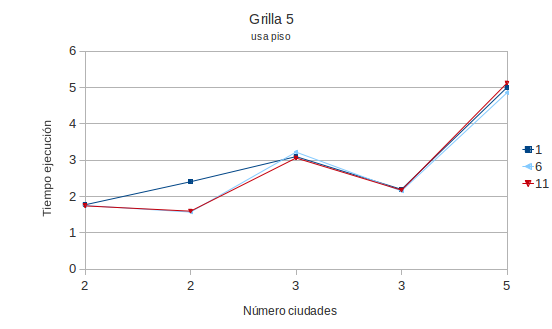
\includegraphics[scale=0.4]{grilla5floor3.png}
 % grilla5ceil3.png: 539x326 pixel, 72dpi, 19.01x11.50 cm, bb=0 0 539 326
 \caption{Comparación mejor heurística}
 \label{fig:grid5floor3}
\end{minipage}
\end{figure}


\newpage
\textbf{Comparación mejor techo-piso}

Tomamos la mejor heurística usando techo y la mejor heurística usando piso, comparamos sus resultados con los ejemplos y concluimos que la mejor era la número $6$, que usaba piso.\\


 
\begin{table}[ht]
\begin{minipage}[b]{1\linewidth}
 \centering
    \begin{tabular}{|c|c|}
        \hline
        6 (PISO)                         & 9 (TECHO)               \\ 
        PSEUDONONINTSELECT               & GREEDY            \\ \hline
        1,753                            & 2,05              \\ \hline
        1,573                            & 1,824             \\ \hline
        3,223                            & 3,993             \\ \hline
        2,154                            & 3,998             \\ \hline
        4,858                            & 6,313             \\
        \hline
    \end{tabular}
    \end{minipage}
\end{table}


\begin{figure}[ht]
\begin{minipage}[b]{1\linewidth}
 \centering
 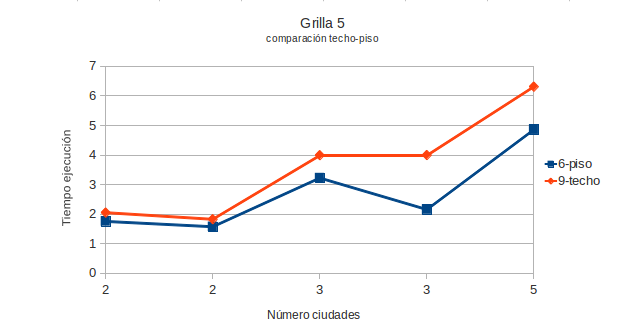
\includegraphics[scale=0.4]{grilla5ceilfloor.png}
 % grilla5ceilfloor.png: 624x328 pixel, 72dpi, 22.01x11.57 cm, bb=0 0 624 328
 \caption{Comparación mejores techo y piso}
 \label{fig:grid5ceilfloor}
 \end{minipage}
\end{figure}

%%FINALIZA GRILLA 5


%%INICIA GRILLA 10

\newpage
\subsection{Ejemplos tamaño de grilla 10}

Gráficas correspondientes al desempeño de las heurísticas, 3 grupos:\\
\textbf{Usando techo:}


\begin{figure}[ht]
\begin{minipage}[b]{0.45\linewidth}
 \centering
 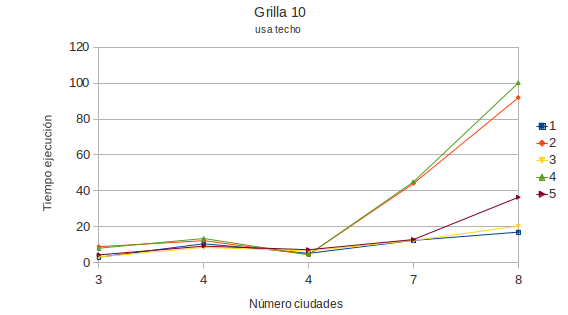
\includegraphics[width=\textwidth]{grilla10ceil0.png}
 % grilla5ceil0.png: 548x330 pixel, 72dpi, 19.33x11.64 cm, bb=0 0 548 330
 \caption{Comparación heurísticas  1 $\cdots$ 5}
 \label{fig:grid10ceil0}
\end{minipage}
\hspace{0.5cm}
\begin{minipage}[b]{0.45\linewidth}
 
\centering
 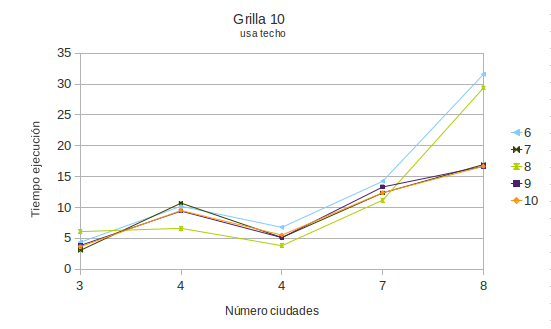
\includegraphics[width=\textwidth]{grilla10ceil1.png}
 % grilla5ceil0.png: 548x330 pixel, 72dpi, 19.33x11.64 cm, bb=0 0 548 330
 \caption{Comparación heurísticas  6 $\cdots$ 10}
 \label{fig:grid10ceil1}
\end{minipage}

\begin{minipage}[b]{1\linewidth}
  \centering
 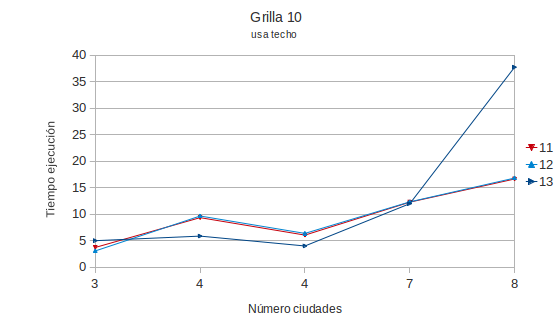
\includegraphics[scale=0.4]{grilla10ceil2.png}
 % grilla5ceil0.png: 548x330 pixel, 72dpi, 19.33x11.64 cm, bb=0 0 548 330
 \caption{Comparación heurísticas  11 $\cdots$ 13}
 \label{fig:grid10ceil2}
\end{minipage}

\end{figure}


De la figura \ref{fig:grid10ceil0} la heurística que presentó mejor desempeño fue la número $1$ (NODE\_FIRSTSELECT), de la figura \ref{fig:grid10ceil1} fue la número $9$ (NODE\_GREEDYMODE) y de la 
figura \ref{fig:grid10ceil2} fue la número $11$ (NODE\_RANDOMIZEMODE). Al comparar éstas tres, la mejor correspondió a la heurística número $11$ (NODE\_RANDOMIZEMODE).

\begin{figure}[ht]
\begin{minipage}[b]{1\linewidth}
 \centering
 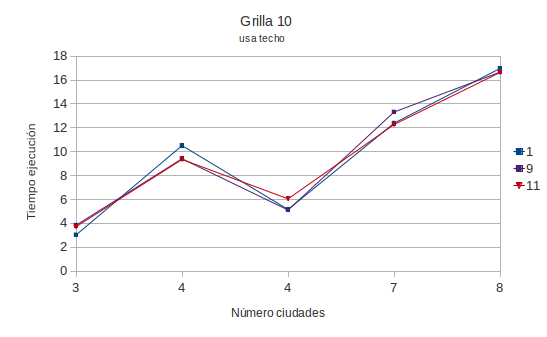
\includegraphics[scale=0.4]{grilla10ceil3.png}
 % grilla5ceil3.png: 539x326 pixel, 72dpi, 19.01x11.50 cm, bb=0 0 539 326
 \caption{Comparación mejor heurística}
 \label{fig:grid10ceil3}
\end{minipage}
\end{figure}

\newpage

\textbf{Usando piso:}

\begin{figure}[ht]

\begin{minipage}[b]{0.45\linewidth}
 \centering
 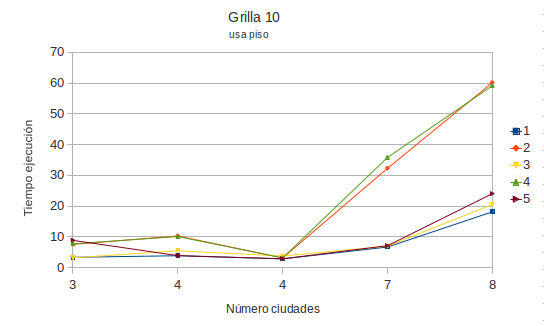
\includegraphics[width=\textwidth]{grilla10floor0.png}
 % grilla5ceil0.png: 548x330 pixel, 72dpi, 19.33x11.64 cm, bb=0 0 548 330
 \caption{Comparación heurísticas  1 $\cdots$ 5}
 \label{fig:grid10floor0}
\end{minipage}
\hspace{0.5cm}
\begin{minipage}[b]{0.45\linewidth}
 \centering
 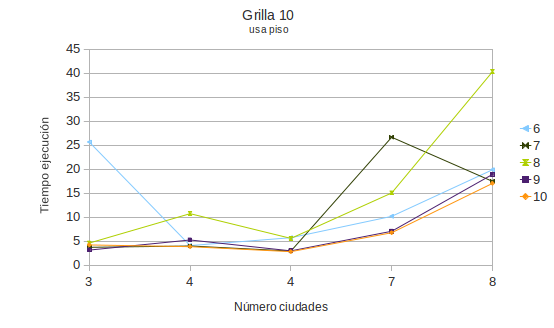
\includegraphics[width=\textwidth]{grilla10floor1.png}
 % grilla5ceil0.png: 548x330 pixel, 72dpi, 19.33x11.64 cm, bb=0 0 548 330
 \caption{Comparación heurísticas  6 $\cdots$ 10}
 \label{fig:grid10floor1}
\end{minipage}

\begin{minipage}[b]{1\linewidth}
  \centering
 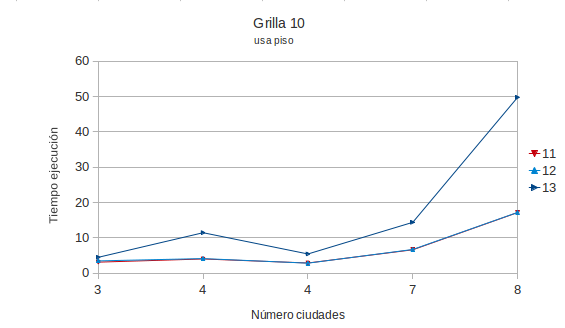
\includegraphics[scale=0.4]{grilla10floor2.png}
 % grilla5ceil0.png: 548x330 pixel, 72dpi, 19.33x11.64 cm, bb=0 0 548 330
 \caption{Comparación heurísticas  11 $\cdots$ 13}
 \label{fig:grid10floor2}
\end{minipage}

\end{figure}


De la figura \ref{fig:grid10floor0} la heurística que presentó mejor desempeño fue la número $1$ (NODE\_FIRSTSELECT), de la figura \ref{fig:grid10floor1} fue la número $10$ (NODE\_DEPTHFIRSTMODE) y de la 
figura \ref{fig:grid10floor2} fue la número $11$ (NODE\_RANDOMIZEMODE). Al comparar éstas tres, la mejor correspondió a la heurística número $10$ (NODE\_DEPTHFIRSTMODE).


\begin{figure}[ht]
\begin{minipage}[b]{1\linewidth}

 \centering
 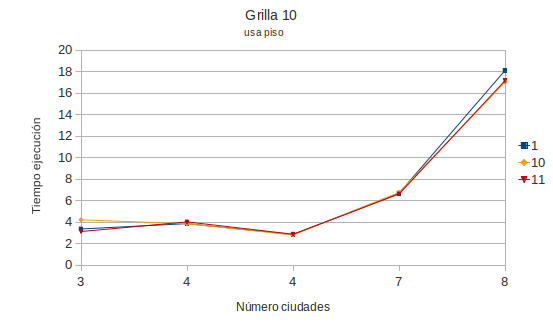
\includegraphics[scale=0.4]{grilla10floor3.png}
 % grilla5ceil3.png: 539x326 pixel, 72dpi, 19.01x11.50 cm, bb=0 0 539 326
 \caption{Comparación mejor heurística}
 \label{fig:grid10floor3}
\end{minipage}
\end{figure}

\newpage

\textbf{Comparación mejor techo-piso}

Tomamos la mejor heurística usando techo y la mejor heurística usando piso, comparamos sus resultados con los ejemplos y concluimos que la mejor era la número $10$, que usaba piso.\\
 
\begin{table}[ht]
\begin{minipage}[b]{1\linewidth}
 \centering
    \begin{tabular}{|c|c|}
        \hline
        10 (PISO)                        & 11 (TECHO)                 \\ 
        DEPTHFIRSTMODE                   & RANDOMIZEMODE            \\ \hline
        4,208                            & 3,719            \\ \hline
        3,849                            & 9,354            \\ \hline
        2,808                            & 6,053             \\ \hline
        6,758                            & 12,279             \\ \hline
        17,041                           & 16,644             \\
        \hline
    \end{tabular}
    \end{minipage}
\end{table}


\begin{figure}[ht]
\begin{minipage}[b]{1\linewidth}
 \centering
 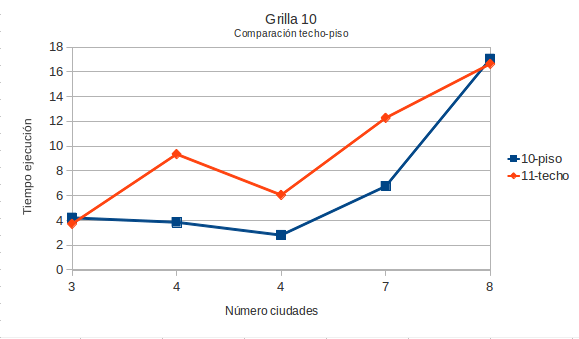
\includegraphics[scale=0.4]{grilla10ceilfloor.png}
 % grilla5ceilfloor.png: 624x328 pixel, 72dpi, 22.01x11.57 cm, bb=0 0 624 328
 \caption{Comparación mejores techo y piso}
 \label{fig:grid10ceilfloor}
 \end{minipage}
\end{figure}

%%FINALIZA GRILLA 10

%%INICIA GRILLA 15
\newpage
\subsection{Ejemplos tamaño de grilla 15}

Gráficas correspondientes al desempeño de las heurísticas, 3 grupos:\\
\textbf{Usando techo:}

\begin{figure}[ht]
\begin{minipage}[b]{0.45\linewidth}
 \centering
 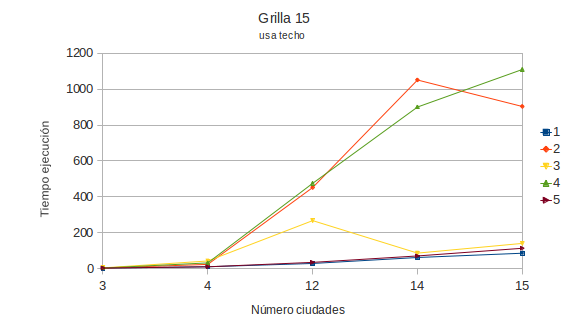
\includegraphics[width=\textwidth]{grilla15ceil0.png}
 % grilla5ceil0.png: 548x330 pixel, 72dpi, 19.33x11.64 cm, bb=0 0 548 330
 \caption{Comparación heurísticas  1 $\cdots$ 5}
 \label{fig:grid15ceil0}
\end{minipage}
\hspace{0.5cm}
\begin{minipage}[b]{0.45\linewidth}
 
\centering
 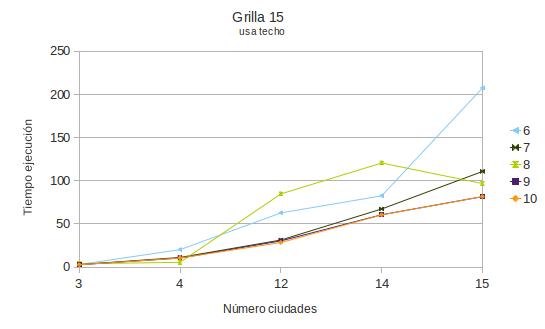
\includegraphics[width=\textwidth]{grilla15ceil1.png}
 % grilla5ceil0.png: 548x330 pixel, 72dpi, 19.33x11.64 cm, bb=0 0 548 330
 \caption{Comparación heurísticas  6 $\cdots$ 10}
 \label{fig:grid15ceil1}
\end{minipage}

\begin{minipage}[b]{1\linewidth}
  \centering
 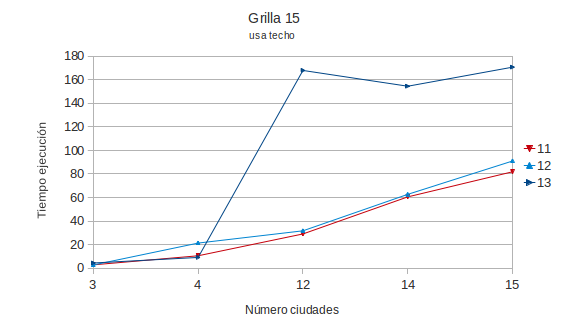
\includegraphics[scale=0.4]{grilla15ceil2.png}
 % grilla5ceil0.png: 548x330 pixel, 72dpi, 19.33x11.64 cm, bb=0 0 548 330
 \caption{Comparación heurísticas  11 $\cdots$ 13}
 \label{fig:grid15ceil2}
\end{minipage}

\end{figure}



De la figura \ref{fig:grid15ceil0} la heurística que presentó mejor desempeño fue la número $1$ (NODE\_FIRSTSELECT), de la figura \ref{fig:grid15ceil1} fue la número $10$ (NODE\_DEPTHFIRSTMODE) y de la 
figura \ref{fig:grid15ceil2} fue la número $11$ (NODE\_RANDOMIZEMODE). Al comparar éstas tres, la mejor correspondió a la heurística número $10$ (NODE\_DEPTHFIRSTMODE).

\begin{figure}[ht]
\begin{minipage}[b]{1\linewidth}
 \centering
 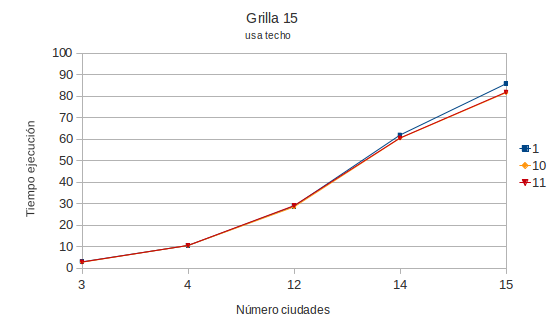
\includegraphics[scale=0.4]{grilla15ceil3.png}
 % grilla5ceil3.png: 539x326 pixel, 72dpi, 19.01x11.50 cm, bb=0 0 539 326
 \caption{Comparación mejor heurística}
 \label{fig:grid15ceil3}
\end{minipage}
\end{figure}


\newpage
\textbf{Usando piso:}

\begin{figure}[ht]

\begin{minipage}[b]{0.45\linewidth}
 \centering
 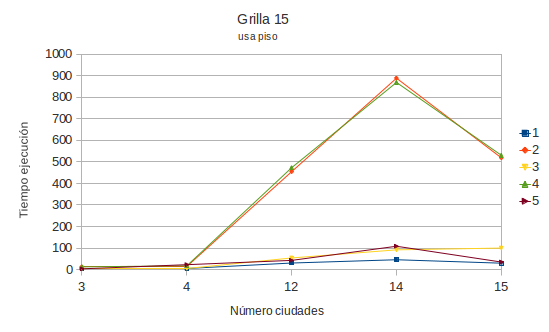
\includegraphics[width=\textwidth]{grilla15floor0.png}
 % grilla5ceil0.png: 548x330 pixel, 72dpi, 19.33x11.64 cm, bb=0 0 548 330
 \caption{Comparación heurísticas  1 $\cdots$ 5}
 \label{fig:grid15floor0}
\end{minipage}
\hspace{0.5cm}
\begin{minipage}[b]{0.45\linewidth}
 \centering
 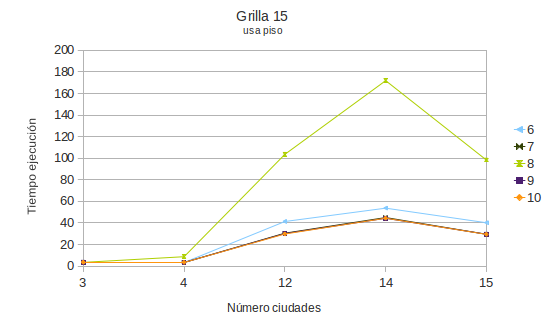
\includegraphics[width=\textwidth]{grilla15floor1.png}
 % grilla5ceil0.png: 548x330 pixel, 72dpi, 19.33x11.64 cm, bb=0 0 548 330
 \caption{Comparación heurísticas  6 $\cdots$ 10}
 \label{fig:grid15floor1}
\end{minipage}

\begin{minipage}[b]{1\linewidth}
  \centering
 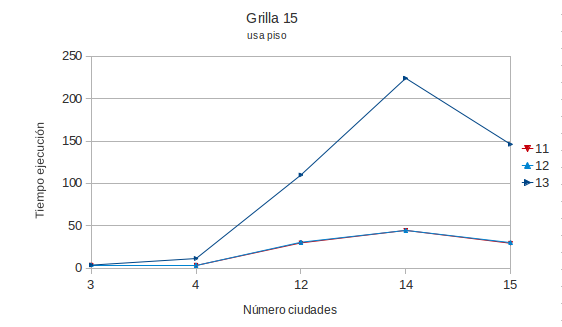
\includegraphics[scale=0.4]{grilla15floor2.png}
 % grilla5ceil0.png: 548x330 pixel, 72dpi, 19.33x11.64 cm, bb=0 0 548 330
 \caption{Comparación heurísticas  11 $\cdots$ 13}
 \label{fig:grid15floor2}
\end{minipage}

\end{figure}


De la figura \ref{fig:grid15floor0} la heurística que presentó mejor desempeño fue la número $1$ (NODE\_FIRSTSELECT), de la figura \ref{fig:grid15floor1} fue la número $10$ (NODE\_DEPTHFIRSTMODE) y de la 
figura \ref{fig:grid15floor2} fue la número $11$ (NODE\_RANDOMIZEMODE). Al comparar éstas tres, la mejor correspondió a la heurística número $10$ (NODE\_DEPTHFIRSTMODE).


\begin{figure}[ht]
\begin{minipage}[b]{1\linewidth}

 \centering
 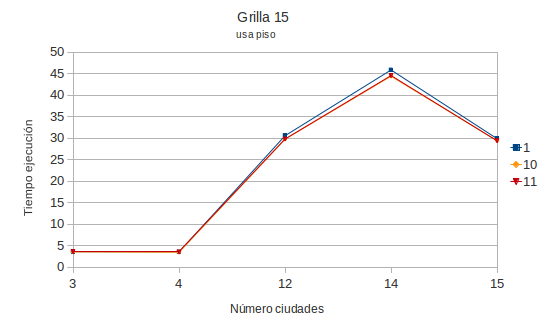
\includegraphics[scale=0.4]{grilla15floor3.png}
 % grilla5ceil3.png: 539x326 pixel, 72dpi, 19.01x11.50 cm, bb=0 0 539 326
 \caption{Comparación mejor heurística}
 \label{fig:grid15floor3}
\end{minipage}
\end{figure}

\newpage
\textbf{Comparación mejor techo-piso}

Tomamos la mejor heurística usando techo y la mejor heurística usando piso, comparamos sus resultados con los ejemplos y concluimos que la mejor era la número $10$, que usaba piso.\\


 
\begin{table}[ht]
\begin{minipage}[b]{1\linewidth}
 \centering
    \begin{tabular}{|c|c|}
        \hline
        10 (PISO)                        & 10 (TECHO)        \\ 
        DEPTHFIRSTMODE                   & DEPTHFIRSTMODE    \\ \hline
        3,526                            & 2,736              \\ \hline
        3,438                            & 10,51             \\ \hline
        29,778                           & 28,466            \\ \hline
        44,423                           & 60,487             \\ \hline
        29,42                            & 81,667             \\
        \hline
    \end{tabular}
    \end{minipage}
\end{table}


\begin{figure}[ht]
\begin{minipage}[b]{1\linewidth}
 \centering
 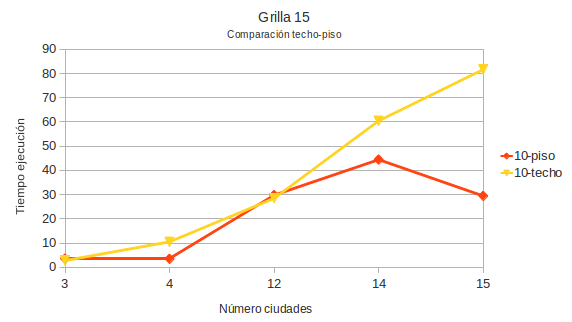
\includegraphics[scale=0.4]{grilla15ceilfloor.png}
 % grilla5ceilfloor.png: 624x328 pixel, 72dpi, 22.01x11.57 cm, bb=0 0 624 328
 \caption{Comparación mejores techo y piso}
 \label{fig:grid15ceilfloor}
 \end{minipage}
\end{figure}

%%FINALIZA GRILLA 15


%%COMIENZA GRILLA 20
\newpage
\subsection{Ejemplos tamaño de grilla 20}

Gráficas correspondientes al desempeño de las heurísticas, 3 grupos:\\
\textbf{Usando techo:}


\begin{figure}[ht]
\begin{minipage}[b]{0.45\linewidth}
 \centering
 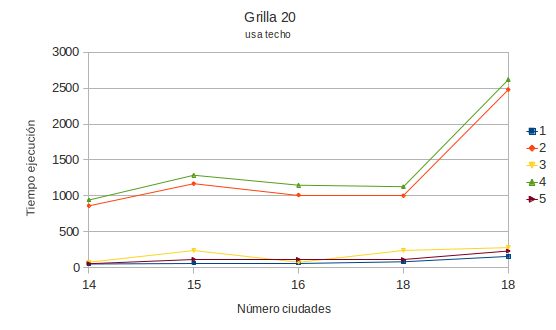
\includegraphics[width=\textwidth]{grilla20ceil0.png}
 % grilla5ceil0.png: 548x330 pixel, 72dpi, 19.33x11.64 cm, bb=0 0 548 330
 \caption{Comparación heurísticas  1 $\cdots$ 5}
 \label{fig:grid20ceil0}
\end{minipage}
\hspace{0.5cm}
\begin{minipage}[b]{0.45\linewidth}
 
\centering
 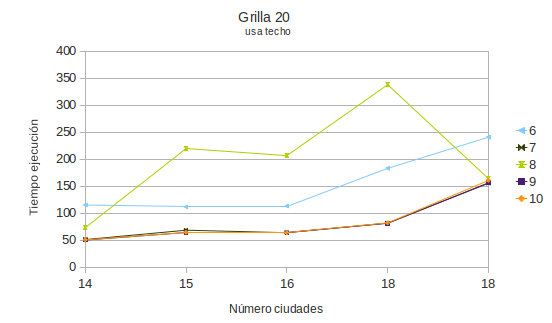
\includegraphics[width=\textwidth]{grilla20ceil1.png}
 % grilla5ceil0.png: 548x330 pixel, 72dpi, 19.33x11.64 cm, bb=0 0 548 330
 \caption{Comparación heurísticas  6 $\cdots$ 10}
 \label{fig:grid20ceil1}
\end{minipage}

\begin{minipage}[b]{1\linewidth}
  \centering
 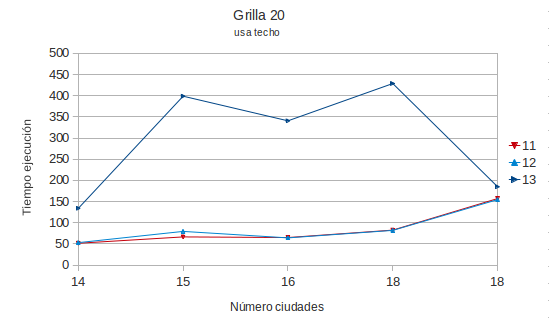
\includegraphics[scale=0.4]{grilla20ceil2.png}
 % grilla5ceil0.png: 548x330 pixel, 72dpi, 19.33x11.64 cm, bb=0 0 548 330
 \caption{Comparación heurísticas  11 $\cdots$ 13}
 \label{fig:grid20ceil2}
\end{minipage}

\end{figure}


De la figura \ref{fig:grid20ceil0} la heurística que presentó mejor desempeño fue la número $1$ (NODE\_FIRSTSELECT), de la figura \ref{fig:grid20ceil1} fue la número $9$ (NODE\_GREEDYMODE) y de la 
figura \ref{fig:grid20ceil2} fue la número $12$ (NODE\_BREADTHFIRSTMODE). Al comparar éstas tres, la mejor correspondió a la heurística número $9$ (NODE\_GREEDYMODE).

\begin{figure}[ht]
\begin{minipage}[b]{1\linewidth}
 \centering
 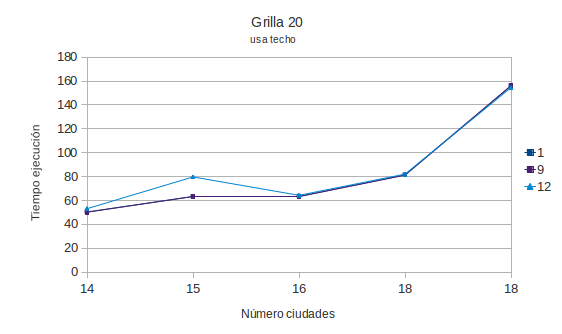
\includegraphics[scale=0.4]{grilla20ceil3.png}
 % grilla5ceil3.png: 539x326 pixel, 72dpi, 19.01x11.50 cm, bb=0 0 539 326
 \caption{Comparación mejor heurística}
 \label{fig:grid20ceil3}
\end{minipage}
\end{figure}

\newpage

\textbf{Usando piso:}

\begin{figure}[ht]

\begin{minipage}[b]{0.45\linewidth}
 \centering
 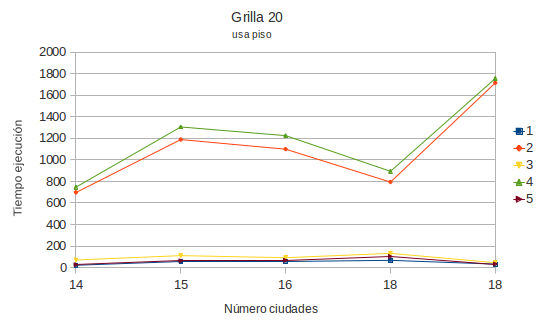
\includegraphics[width=\textwidth]{grilla20floor0.png}
 % grilla5ceil0.png: 548x330 pixel, 72dpi, 19.33x11.64 cm, bb=0 0 548 330
 \caption{Comparación heurísticas  1 $\cdots$ 5}
 \label{fig:grid20floor0}
\end{minipage}
\hspace{0.5cm}
\begin{minipage}[b]{0.45\linewidth}
 \centering
 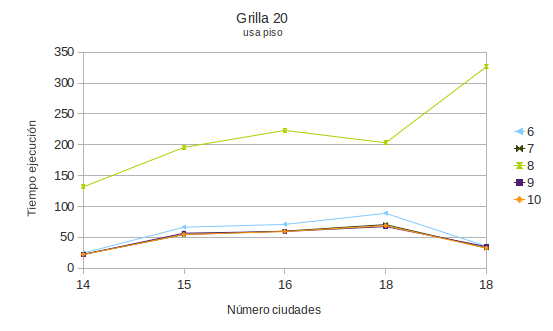
\includegraphics[width=\textwidth]{grilla20floor1.png}
 % grilla5ceil0.png: 548x330 pixel, 72dpi, 19.33x11.64 cm, bb=0 0 548 330
 \caption{Comparación heurísticas  6 $\cdots$ 10}
 \label{fig:grid20floor1}
\end{minipage}

\begin{minipage}[b]{1\linewidth}
  \centering
 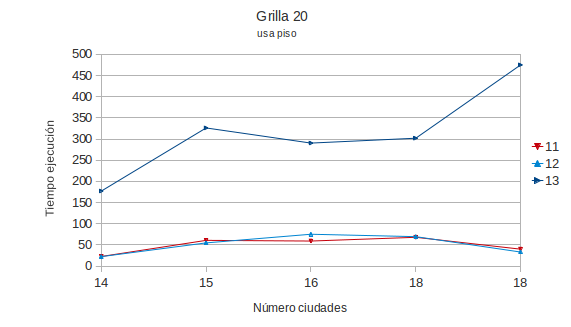
\includegraphics[scale=0.4]{grilla20floor2.png}
 % grilla5ceil0.png: 548x330 pixel, 72dpi, 19.33x11.64 cm, bb=0 0 548 330
 \caption{Comparación heurísticas  11 $\cdots$ 13}
 \label{fig:grid20floor2}
\end{minipage}

\end{figure}


De la figura \ref{fig:grid20floor0} la heurística que presentó mejor desempeño fue la número $1$ (NODE\_FIRSTSELECT), de la figura \ref{fig:grid20floor1} fue la número $10$ (NODE\_DEPTHFIRSTMODE) y de la 
figura \ref{fig:grid20floor2} fue la número $12$ (NODE\_BREADTHFIRSTMODE). Al comparar éstas tres, la mejor correspondió a la heurística número $1$ (NODE\_FIRSTSELECT).


\begin{figure}[ht]
\begin{minipage}[b]{1\linewidth}

 \centering
 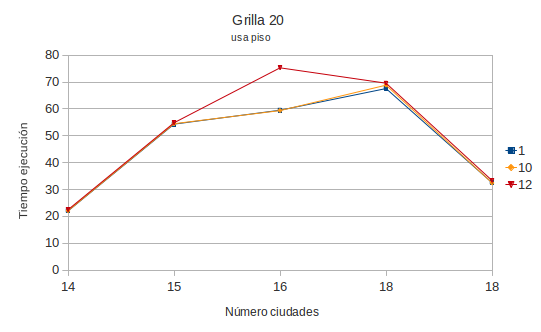
\includegraphics[scale=0.4]{grilla20floor3.png}
 % grilla5ceil3.png: 539x326 pixel, 72dpi, 19.01x11.50 cm, bb=0 0 539 326
 \caption{Comparación mejor heurística}
 \label{fig:grid20floor3}
\end{minipage}
\end{figure}

\newpage
\textbf{Comparación mejor techo-piso}

Tomamos la mejor heurística usando techo y la mejor heurística usando piso, comparamos sus resultados con los ejemplos y concluimos que la mejor era la número $1$, que usaba piso.\\


 
\begin{table}[ht]
\begin{minipage}[b]{1\linewidth}
 \centering
    \begin{tabular}{|c|c|}
        \hline
        1 (PISO)                         & 9 (TECHO)         \\ 
        FIRSTSELECT                      & GREEDY            \\ \hline
        22,027                           & 50,166              \\ \hline
        54,355                           & 63,448             \\ \hline
        59,531                           & 63,413             \\ \hline
        67,59                            & 81,275             \\ \hline
        32,537                           & 156,267             \\
        \hline
    \end{tabular}
    \end{minipage}
\end{table}


\begin{figure}[ht]
\begin{minipage}[b]{1\linewidth}
 \centering
 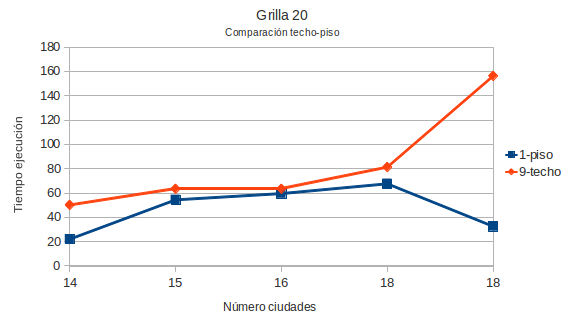
\includegraphics[scale=0.4]{grilla20ceilfloor.png}
 % grilla5ceilfloor.png: 624x328 pixel, 72dpi, 22.01x11.57 cm, bb=0 0 624 328
 \caption{Comparación mejores techo y piso}
 \label{fig:grid20ceilfloor}
 \end{minipage}
\end{figure}

%%FINALIZA GRILLA 20



%%COMPARACIÓN TODS LAS HEURISTICAS EN FLOOR
\newpage
\subsection{Comparación todas las heurísticas usando piso}
Como se evidencia en las gráficas anteriores, las heurísticas tuvieron mejor desempeño cuando usaban la función piso. Es por ello que para poder obtener las tres mejores heurísticas del
B\&B para nuestro modelo, comparamos todas las heurísticas usando la función piso con un ejemplo de cada una de las grillas (se eligió el ejemplo con mayor número de ciudades). Nuevamente
graficamos el desempeño de las heurísticas en 3 grupos, seleccionamos las tres mejores y finalmente se plantea las conclusiones.

\begin{figure}[ht]

\begin{minipage}[b]{0.45\linewidth}
 \centering
 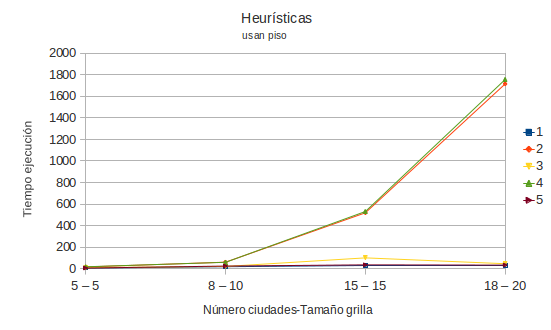
\includegraphics[width=\textwidth]{heuristicas0.png}
 % grilla5ceil0.png: 548x330 pixel, 72dpi, 19.33x11.64 cm, bb=0 0 548 330
 \caption{Comparación heurísticas  1 $\cdots$ 5}
 \label{fig:heu0}
\end{minipage}
\hspace{0.5cm}
\begin{minipage}[b]{0.45\linewidth}
 \centering
 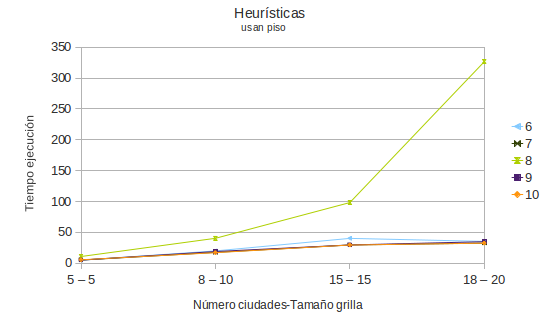
\includegraphics[width=\textwidth]{heuristicas1.png}
 % grilla5ceil0.png: 548x330 pixel, 72dpi, 19.33x11.64 cm, bb=0 0 548 330
 \caption{Comparación heurísticas  6 $\cdots$ 10}
 \label{fig:heu1}
\end{minipage}

\begin{minipage}[b]{1\linewidth}
  \centering
 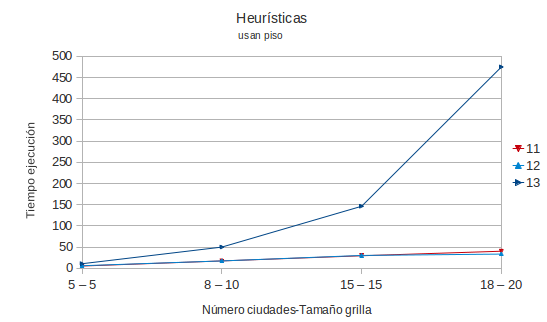
\includegraphics[scale=0.4]{heuristicas2.png}
 % grilla5ceil0.png: 548x330 pixel, 72dpi, 19.33x11.64 cm, bb=0 0 548 330
 \caption{Comparación heurísticas  11 $\cdots$ 13}
 \label{fig:heu2}
\end{minipage}

\end{figure}

Finalmente comparamos la mejor heurística de cada grupo.

\begin{figure}[ht]
\begin{minipage}[b]{1\linewidth}
 \centering
 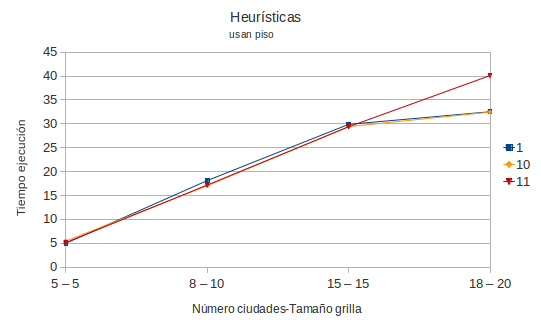
\includegraphics[scale=0.4]{heuristicas3.png}
 % grilla5ceilfloor.png: 624x328 pixel, 72dpi, 22.01x11.57 cm, bb=0 0 624 328
 \caption{Comparación mejores heurísticas}
 \label{fig:heu3}
 \end{minipage}
\end{figure}

\newpage

Concluimos que la heurística que obtuvo un mejor desempeño fue la número $10$ (NODE\_DEPTHFIRSTMODE) y es la heurística que finalmente usamos para resolver el problema.\\

La función piso tuvo mejor comportamiento que la función techo en las heurísticas, y es por que nuestro modelo requería que solo una variable binaria de un conjunto tomará el 
valor de 1. Las variables binarias fueron usadas como flags de las restricciones. Por ello probar con que una variable tomara primero el valor de $0$ resultó mas efectivo. \\

De las tres mejores heurísticas se destaca la opción de no perder tanto tiempo en que rama elegir sino en proceder con los subproblemas generados. Puesto que una vez se tiene activado
la función piso, se debe de buscar de manera más rápida el valor de las otras variables no-enteras.\\

Heurísticas como la número $2$, $4$, $8$ y $13$ perdían mucho tiempo tratando de optimizar la variable a escoger, sin llegar rápido a la solución. Esto se debe a que debían realizar
comparaciones de costos de cada una de las ramas para determinar por cual seguir.\\

\newpage
\section{Implementaci\'on}

Para la implementaci\'on del modelo presentado anteriormente usamos el programa lpSolver, lpSolver es un programa para resolver problemas de programación lineal y programación entera.\\

LpSolver es un programa de código abierto licencia LGPL basado en el método simplex para resolver problemas de programación lineal y en el método branch and bound para resolver problemas de programaci\'on entera.\\

Usamos además la librería de LpSolver para java, puesto que éste fue nuestro lenguaje de programación. El proyecto fue desarrollado en Netbeans, se cuenta con una interfaz gráfica que permite
ver la solución encontrada.\\

Un ejemplo de la implementación de una restricción es dado a continuación, lp corresponde al modelo en LpSolver:\\

\begin{lstlisting}[language=Java]
// restricciones obvias Xb <= sizeGrid y Yb <= sizeGrid y
        // Xc <= sizeGrid y Yc <= sizeGrid
        for (int i = 0; i < 2; i++) {

            int[] colno = new int[Ncol];
            double[] row = new double[Ncol];

            colno[ i + posDump] = 1 + i + posDump;
            row[ i + posDump] = 1;

            lp.addConstraintex(Ncol, row, colno, LpSolve.LE, sizeGrid);

            colno = new int[Ncol];
            row = new double[Ncol];

            colno[ i + posNearbyCity] = 1 + i + posNearbyCity;
            row[ i + posNearbyCity] = 1;

            lp.addConstraintex(Ncol, row, colno, LpSolve.LE, sizeGrid); //Se añade la restricción al modelo

        }
\end{lstlisting}

Para realizar las pruebas se realizó una clase que generara los archivos de prueba (.txt) y para obtener los datos de solución y desempeño se generaron archivos (.csv). Para ver estos
archivos por favor revisar las carpetas (analisis\_heuristicas) y (src/Solver/ejemplos\_g\_e) respectivamente.

\newpage
\section{Conclusiones}
\begin{itemize}
 \item Al poder modelar un problema usando Programación Lineal se permite encontrar soluciones optimas de manera mas rapida que usando otros tipos de paradigma
Sabiendo esto, la dificultad esta en plantear dicho modelo es por ello que la mayor inversión de tiempo en la programación LP se lleva acabo en el desarrollo del modelo matemático. Es este el que le da el soporte a las restricciones para que un problema
pueda ser resuelto mas adelante con alguna implementación. Por lo cual un mal planteamiento puede que solo encuentre soluciones parciales que pueden ser buenas pero que no son las 
óptimas o por el contrario arroja resultados incorrectos para ciertos casos.
\item Las restricciones \emph{obvias} resultan de mucha importancia, pues acotan los espacios de búsqueda y establecen condiciones que de otra manera podrían ser violadas eventualmente. 
Un ejemplo de esto es la restricción que declara que la ciudad mas cercana (variable) debe pertenecer al conjunto de ciudades descritas en el problema.
\item Diferentes heurísticas del B\&B pueden darnos algunos resultados con variables con diferentes valores pero con la función objetivo igual, esto nos dice que conociendo bien el problema
y las heurísticas a usar podríamos obtener un conjunto de soluciones óptimas para evaluar eventualmente cual sería una mejor solución para nuestro problema. Por ejemplo una ciudad cercana
que colocara mas condiciones por construir el basurero tan cerca, de otra cuyas condiciones son menores, pero donde la función objetivo se mantiene.
\item La heurística a elegir para el B\&B depende en gran medida del modelo en particular. Pues una búsqueda que para un modelo resulte efectiva en otro puede ser mucho mas costosa y 
afectar los tiempo de respuesta. Es por ello que se debe analizar el modelo desarrollado y seleccionar las heurísticas mas adecuadas.
\item La librería para java LpSolve permite implementar modelos de Programación Lineal con mayor fluidez. Esto ayuda a enfocarse mas en las restricciones que se están escribiendo que en cómo 
hacer restricciones en java. Enfocarse mas en el qué que en el cómo.
\end{itemize}



\end{document}
